\documentclass[a4paper,oneside,11pt]{book}
	
\usepackage[spanish]{babel}
\usepackage[utf8]{inputenc}

% -------------------------------------------------------------------------

% Para incluir graficos en JPG => compilar con pdflatex.
%\usepackage[pdftex]{graphicx}
% Para incluir graficos EPS => compilar con latex.
\usepackage[dvips]{graphicx}
% Para escribir en color cuando compilamos con pdflatex
\usepackage[pdftex,usenames,dvipsnames]{color}

% -------------------------------------------------------------------------

% Paquete fancyhdr -> Para modificar la cabecera y pie de paginas.
% http://tug.ctan.org/tex-archive/macros/latex/contrib/fancyhdr/
\usepackage{fancyhdr}
\pagestyle{fancy}
\fancyhf{}
\fancyhf[HR]{\thepage}
\fancyhf[HL]{\nouppercase\rightmark}
\headwidth=16cm

% Ajuste de margenes
\usepackage{anysize}
\marginsize{3cm}{2cm}{2cm}{2cm}	% izquierda, derecha, arriba, abajo
\parskip=6pt	% Personalizamos la separacion entre parrafos.
\parindent=10pt	% Personalizamos el identado en la primera linea del nuevo parrafo.
\setcounter{secnumdepth}{3}	% Numero maximo de niveles de profundidad en las secciones.

% -------------------------------------------------------------------------

% Package booktabs -> Para mejorar el aspecto de las tablas o cuadros.
% http://www.ctan.org/tex-archive/macros/latex/contrib/booktabs/
\usepackage{booktabs}

% Package rotating -> Para poder girar las tablas y dibujarlas a lo largo
% del folio en vez de a lo ancho.
\usepackage{rotating}

% Packages multicol y multirow, para manejar tablas de filas y columnas multiples.
\usepackage{multicol}
\usepackage{multirow}

\usepackage{tabularx}

% -------------------------------------------------------------------------
% Compilar con bibtex book.gls.aux
\usepackage[refpages]{gloss}
% -------------------------------------------------------------------------

\title{Desarrollo Aplicación Web de Gestión Deportiva para Entrenadores de Natación}
\author{Roberto Marco Sánchez}
\date{\today}

\begin{document}
	\maketitle
	\makegloss
	
	% FRONTMATTER: TOC, LOF, LOT y descripcion/organizacion de la memoria.
	\frontmatter

	\tableofcontents
	\listoffigures
	\listoftables
	%
% Frontmatter - Introducci�n. Los miembros del tribunal que juzgan los PFC's tienen muchas m�s memorias que leer, por lo que
%	agradecer�n cualquier detalle que permita facilitarles la vida. En este sentido, realizar una peque�a introducci�n,
%	comentar la organizaci�n y estructura de la memoria y resumir brevemente cada cap�tulo puede ser una buena pr�ctica
%	que permita al lector centrarse f�cilmente en la parte que m�s le interesa.
%

\chapter[Introducci�n]{
	Introducci�n
}

La introducci�n es lo primero que se lee, pero habitualmente lo �ltimo que se escribe.
Pues su redacci�n depende de c�mo se hayan escrito todas las otras secciones. Normalmente la introducci�n incluye una descripci�n muy general del proyecto y termina con un desglose del contenido de la memoria.

One for all and all for one, Muskehounds are always ready. One for all and all for one, helping everybody. One for all and all for one, it's a pretty story. Sharing everything with fun, that's the way to be. One for all and all for one, Muskehounds are always ready. One for all and all for one, helping everybody. One for all and all for one, can sound pretty corny. If you've got a problem chum, think how it could be.

Hong Kong Phooey, number one super guy. Hong Kong Phooey, quicker than the human eye. He's got style, a groovy style, and a car that just won't stop. When the going gets tough, he's really rough, with a Hong Kong Phooey chop (Hi-Ya!). Hong Kong Phooey, number one super guy. Hong Kong Phooey, quicker than the human eye. Hong Kong Phooey, he's fan-riffic!

Ten years ago a crack commando unit was sent to prison by a military court for a crime they didn't commit. These men promptly escaped from a maximum security stockade to the Los Angeles underground. Today, still wanted by the government, they survive as soldiers of fortune. If you have a problem and no one else can help, and if you can find them, maybe you can hire the A-team.

This is my boss, Jonathan Hart, a self-made millionaire, he's quite a guy. This is Mrs H., she's gorgeous, she's one lady who knows how to take care of herself. By the way, my name is Max. I take care of both of them, which ain't easy, 'cause when they met it was MURDER!

Top Cat! The most effectual Top Cat! Who's intellectual close friends get to call him T.C., providing it's with dignity. Top Cat! The indisputable leader of the gang. He's the boss, he's a pip, he's the championship. He's the most tip top, Top Cat.

%
% SECCION
%
\subsection*{Estructura de la memoria}


In a dolor sed odio eleifend varius. Nam ullamcorper. Curabitur ut erat vulputate nisi molestie tempus. Sed aliquam rutrum odio. In mollis. Fusce consectetuer lorem nec diam. Sed mollis lacinia purus. Curabitur feugiat hendrerit neque. Quisque auctor laoreet diam. Curabitur sit amet nisi. Fusce velit massa, dignissim quis, bibendum eget, vehicula mattis, leo. Morbi auctor leo sit amet nibh. Lorem ipsum dolor sit amet, consectetuer adipiscing elit. Nullam enim. Pellentesque hendrerit, augue non vulputate semper, sem lorem pharetra nibh, sit amet egestas massa diam ac augue. In dui nulla, egestas nec, pulvinar suscipit, tincidunt ornare, nisi. Duis tristique tortor quis magna. Vestibulum faucibus lorem nec neque. Sed nec nibh. Nunc condimentum. Maecenas neque. Nullam pretium est non risus. Etiam gravida. Maecenas nisl. Fusce pharetra odio in tortor. Integer orci turpis, interdum eget, vulputate sed, tristique a, metus. Duis vitae dui quis lectus pretium aliquam. Praesent quam.

Aliquam sed orci. Cras adipiscing nisl quis pede. Ut rhoncus. Donec viverra laoreet purus. Phasellus nulla. Vivamus eget eros. In mollis aliquam orci. Proin ullamcorper. Nullam sollicitudin vestibulum lorem. Nunc malesuada sagittis augue. Donec tellus velit, dapibus a, aliquam ac, tincidunt id, lectus. 


\paragraph*{Cap�tulo 1.}
Phasellus tempor velit nec velit. Proin vitae dui a sapien commodo blandit. Etiam aliquam, sapien vitae fringilla venenatis, lectus sem accumsan orci, eget blandit orci odio et magna. Quisque malesuada, eros vel tempus eleifend, velit enim porttitor sem, eget consequat nulla neque et sapien. Morbi leo. Sed vestibulum lacus. Fusce ut lacus. Phasellus pellentesque pede eu eros. Duis turpis felis, eleifend ut, semper ac, porta nec, sem. Praesent odio. Sed laoreet mollis purus. Praesent vestibulum, velit ut mollis aliquam, quam lectus varius urna, sed ultricies erat nisl ac tortor. Vivamus tempor mauris sit amet nulla. Integer venenatis. Integer sagittis euismod ante. Suspendisse at elit. Duis eget purus nec pede adipiscing auctor. Proin ac est.

\paragraph*{Cap�tulo 2.}
Proin condimentum. Maecenas sodales. In ornare nunc a leo. Nam sit amet ligula. Nunc quis urna ac metus imperdiet lobortis. Sed quis ligula. Maecenas blandit pede. Donec lacinia rutrum ligula. Vivamus in metus vel elit pharetra molestie.

\paragraph*{Cap�tulo 3.}
Nullam ante lorem, placerat et, egestas nec, pellentesque non, sapien. Donec semper, felis id posuere faucibus, nibh ipsum tincidunt quam, et varius ipsum odio ac neque. In tincidunt dignissim diam. Sed lacus lorem, ornare ut, eleifend vel, pellentesque tempus, augue. Duis eu magna. Mauris libero ante, porttitor vel, lobortis a, mollis ac, sem. Nunc at lectus. Integer ac libero a nisl dignissim mollis. Donec velit neque, vestibulum eget, pulvinar vel, malesuada ut, nisi. Praesent congue tempus quam. Cum sociis natoque penatibus et magnis dis parturient montes, nascetur ridiculus mus.

\paragraph*{Cap�tulo 4.}
Mauris ut odio. Nulla accumsan. Morbi condimentum fermentum purus. Pellentesque habitant morbi tristique senectus et netus et malesuada fames ac turpis egestas. Nunc dignissim, neque eget convallis pretium, diam tortor fringilla lacus, a laoreet nisl metus eu magna. Cras ut lectus. Etiam accumsan feugiat elit.

\paragraph*{Cap�tulo ...}
Donec a pede. Proin dolor. Ut nunc ligula, tempor id, ornare sit amet, aliquam et, nibh. In mollis iaculis pede. Vivamus gravida orci eu nisl. Sed nibh sem, consequat at, iaculis non, placerat in, ligula. Praesent id nisi. Nunc pellentesque justo non libero. Sed quis est sit amet purus lobortis blandit. Sed arcu justo, rhoncus condimentum, ullamcorper iaculis, viverra et, nisl.

\paragraph*{Cap�tulo N.}
Fusce luctus gravida leo. Nullam dignissim arcu ac risus hendrerit rhoncus. Aliquam erat volutpat. Ut mollis, mauris non aliquam luctus, nulla sem aliquam tellus, in consequat augue odio in urna.

%
% SECCION
%
\subsection*{Estructura de la memoria}


In a dolor sed odio eleifend varius. Nam ullamcorper. Curabitur ut erat vulputate nisi molestie tempus. Sed aliquam rutrum odio. In mollis. Fusce consectetuer lorem nec diam. Sed mollis lacinia purus. Curabitur feugiat hendrerit neque. Quisque auctor laoreet diam. Curabitur sit amet nisi. Fusce velit massa, dignissim quis, bibendum eget, vehicula mattis, leo. Morbi auctor leo sit amet nibh. Lorem ipsum dolor sit amet, consectetuer adipiscing elit. Nullam enim. Pellentesque hendrerit, augue non vulputate semper, sem lorem pharetra nibh, sit amet egestas massa diam ac augue. In dui nulla, egestas nec, pulvinar suscipit, tincidunt ornare, nisi. Duis tristique tortor quis magna. Vestibulum faucibus lorem nec neque. Sed nec nibh. Nunc condimentum. Maecenas neque. Nullam pretium est non risus. Etiam gravida. Maecenas nisl. Fusce pharetra odio in tortor. Integer orci turpis, interdum eget, vulputate sed, tristique a, metus. Duis vitae dui quis lectus pretium aliquam. Praesent quam.

Aliquam sed orci. Cras adipiscing nisl quis pede. Ut rhoncus. Donec viverra laoreet purus. Phasellus nulla. Vivamus eget eros. In mollis aliquam orci. Proin ullamcorper. Nullam sollicitudin vestibulum lorem. Nunc malesuada sagittis augue. Donec tellus velit, dapibus a, aliquam ac, tincidunt id, lectus. 


\paragraph*{Cap�tulo 1.}
Phasellus tempor velit nec velit. Proin vitae dui a sapien commodo blandit. Etiam aliquam, sapien vitae fringilla venenatis, lectus sem accumsan orci, eget blandit orci odio et magna. Quisque malesuada, eros vel tempus eleifend, velit enim porttitor sem, eget consequat nulla neque et sapien. Morbi leo. Sed vestibulum lacus. Fusce ut lacus. Phasellus pellentesque pede eu eros. Duis turpis felis, eleifend ut, semper ac, porta nec, sem. Praesent odio. Sed laoreet mollis purus. Praesent vestibulum, velit ut mollis aliquam, quam lectus varius urna, sed ultricies erat nisl ac tortor. Vivamus tempor mauris sit amet nulla. Integer venenatis. Integer sagittis euismod ante. Suspendisse at elit. Duis eget purus nec pede adipiscing auctor. Proin ac est.

\paragraph*{Cap�tulo 2.}
Proin condimentum. Maecenas sodales. In ornare nunc a leo. Nam sit amet ligula. Nunc quis urna ac metus imperdiet lobortis. Sed quis ligula. Maecenas blandit pede. Donec lacinia rutrum ligula. Vivamus in metus vel elit pharetra molestie.

\paragraph*{Cap�tulo 3.}
Nullam ante lorem, placerat et, egestas nec, pellentesque non, sapien. Donec semper, felis id posuere faucibus, nibh ipsum tincidunt quam, et varius ipsum odio ac neque. In tincidunt dignissim diam. Sed lacus lorem, ornare ut, eleifend vel, pellentesque tempus, augue. Duis eu magna. Mauris libero ante, porttitor vel, lobortis a, mollis ac, sem. Nunc at lectus. Integer ac libero a nisl dignissim mollis. Donec velit neque, vestibulum eget, pulvinar vel, malesuada ut, nisi. Praesent congue tempus quam. Cum sociis natoque penatibus et magnis dis parturient montes, nascetur ridiculus mus.

\paragraph*{Cap�tulo 4.}
Mauris ut odio. Nulla accumsan. Morbi condimentum fermentum purus. Pellentesque habitant morbi tristique senectus et netus et malesuada fames ac turpis egestas. Nunc dignissim, neque eget convallis pretium, diam tortor fringilla lacus, a laoreet nisl metus eu magna. Cras ut lectus. Etiam accumsan feugiat elit.

\paragraph*{Cap�tulo ...}
Donec a pede. Proin dolor. Ut nunc ligula, tempor id, ornare sit amet, aliquam et, nibh. In mollis iaculis pede. Vivamus gravida orci eu nisl. Sed nibh sem, consequat at, iaculis non, placerat in, ligula. Praesent id nisi. Nunc pellentesque justo non libero. Sed quis est sit amet purus lobortis blandit. Sed arcu justo, rhoncus condimentum, ullamcorper iaculis, viverra et, nisl.

\paragraph*{Cap�tulo N.}
Fusce luctus gravida leo. Nullam dignissim arcu ac risus hendrerit rhoncus. Aliquam erat volutpat. Ut mollis, mauris non aliquam luctus, nulla sem aliquam tellus, in consequat augue odio in urna.



	
	% MAINMATTER: El contenido, capitulo a capitulo, de la memoria.
	\mainmatter

	% ----------------------------------
% Cap Captura de Requisitos
% ----------------------------------
%
%	- Comenzar el capítulo hablando sobre el desarrollo de aplicaciones por un ingeniero. 
%	Es un proceso complicado en el que se localiza primero las necesidades del cliente, 
%	usando una lista de características. Esta lista de características va a servir al jefe 
%	de proyecto en la guía a la construcción del sistema final. 
%	Al finalizar el proyecto, todas las características que están con Estado = Aceptado, 
%	tienen que estar en Estado = Finalizado.
%	Las características se dividirán en iteraciones e incrementos.
%

\chapter{Captura de requisitos} % (fold)
\label{cha:captura_de_requisitos}
	
	En este apartado se describe de forma detallada cada una de las funcionalidades que pueden componer el proyecto, con el fin de guiar el desarrollo hacia el sistema correcto. El proceso estará apoyado en una lista de características y en el modelo del dominio.

% 
% Sec Tipos de usuarios
%
\section{Tipos de usuarios} % (fold)
	\label{sec:tipos_de_usuarios}
	
	Inicialmente se realiza una clasificación de los posibles usuarios del sistema. Esta primera aproximación sólo sirve para identificar y asociar cada característica con cada uno de los usuarios.

	\begin{itemize}
		\item {{\bf Navegante}. Usuario que accederá a las interfaces públicas de la aplicación. Entiéndase como interfaz pública aquella que no necesita registro y autenticación para acceder.}
		\item {{\bf Entrenador}. Usuario destino de la aplicación, con la capacidad de poder acceder al sistema y usar todas las funcionalidades del mismo.}
		\item {{\bf Administrador del sistema}. Es el encargado de configurar la aplicación. Podrá asignar permisos a usuarios en el caso de que exista una gestión de usuarios.}
		\item {{\bf Desarrollador}. La aplicación podrá informar a los desarrolladores de ciertos aspectos como, por ejemplo, informes de errores, mejoras que deseen los usuarios o estadísticas del rendimiento de la aplicación. También se podrá ejecutar en un entorno de depuración, de forma que se puedan detectar aspectos a corregir y mejorar.}
	\end{itemize}

	Posteriormente, cuando se empiece con el desarrollo formal del proyecto, se identificarán los usuarios definitivos, que no tienen por qué coincidir con los propuestos en esta sección.
	
% section tipos_de_usuarios (end)

% 
% Sec Lista de características
%
\section{Lista de características} % (fold)
	\label{sec:lista_de_caracteristicas}
	
	Cada característica tiene un nombre corto y una breve explicación, información suficiente para poder hablar de ella durante la planificación del producto. Cada característica tiene también un conjunto de valores de planificación que son incluidos:
	
	\begin{itemize}
		\item{{\bf Prioridad}. Se asigna una prioridad a cada característica con el fin de determinar el orden en que se van a ir desarrollando. La prioridad se establece desde muy alta a muy baja.}
		\item{{\bf Estado}. Establece el punto en que se encuentra el sistema a medida que avanza su desarrollo. Los posibles estados son: {\it aceptado}, que indica que la característica se desarrollará en esta versión del producto; {\it planificado}, donde se indica que una característica ha sido planificada y se empezará a desarrollar en un plazo de tiempo corto; {\it en desarrollo}; {\it finalizado}; {\it postergado}, que refleja que no se desarrollará hasta una versión futura; y {\it rechazado}, lo que hará que posiblemente no se desarrolle en ninguna versión.}
		\item{{\bf Coste}. Recursos estimados para la implementación de la característica.}
		\item{{\bf Nivel de riesgo asociado}. Cada característica puede tener asociado un riesgo que representa la dificultad para conseguir implementarla correctamente. Los tres niveles de riesgo son: {\it crítico, significativo o rutinario}.}
	\end{itemize}
	
	Para una mayor facilidad en la catalogación, la lista de características está dividida por categorías que representan una aproximación a los módulos que compondrán el sistema.
%
% Sub Navegación (A)
%
\subsection{Navegación(A)} % (fold)
	\label{sub:lc_navegacion}
	
	\begin{center}
		\begin{tabularx}{15cm}{|X|}
			\hline 
				\bf{LC-A1. Tour de la aplicación}\\
			\hline
				Se debe mostrar una página estática como interfaz de entrada con un tour de las características de la aplicación, mostrando la potencia de la misma. Se incluyen páginas acerca de cada uno de los módulos que se gestionan y capturas de pantalla de las mismas.\\
			\hline
				{\it Prioridad} - Bajo\\
			\hline
				{\it Estado} - Aceptado\\
			\hline
				{\it Coste}\\
			\hline
				{\it Riesgo} - Rutinario\\
			\hline
		\end{tabularx}
	\end{center}
	
	\begin{center}
		\begin{tabularx}{15cm}{|X|}
			\hline 
				\bf{LC-A2. Términos legales}\\
			\hline
				El sistema debe mostrar una página estática con los términos.\\
			\hline
				{\it Prioridad} - Bajo\\
			\hline
				{\it Estado} - Aceptado\\
			\hline
				{\it Coste}\\
			\hline
				{\it Riesgo} - Rutinario\\
			\hline
		\end{tabularx}
	\end{center}
	
	\begin{center}
		\begin{tabularx}{15cm}{|X|}
			\hline 
				\bf{LC-A3. Condiciones de uso}\\
			\hline
				El sistema debe mostrar una página estática con las condiciones de uso y privacidad de información.\\
			\hline
				{\it Prioridad} - Bajo\\
			\hline
				{\it Estado} - Aceptado\\
			\hline
				{\it Coste}\\
			\hline
				{\it Riesgo} - Rutinario\\
			\hline
		\end{tabularx}
	\end{center}
	
	\begin{center}
		\begin{tabularx}{15cm}{|X|}
			\hline 
				\bf{LC-A3. Condiciones de uso}\\
			\hline
				El sistema debe mostrar una página estática con las condiciones de uso y privacidad de información.\\
			\hline
				{\it Prioridad} - Bajo\\
			\hline
				{\it Estado} - Aceptado\\
			\hline
				{\it Coste}\\
			\hline
				{\it Riesgo} - Rutinario\\
			\hline
		\end{tabularx}
	\end{center}
	
	\begin{center}
		\begin{tabularx}{15cm}{|X|}
			\hline 
				\bf{LC-A4. Referencias a la aplicación}\\
			\hline
				Se muestra una página estática con las referencias al producto realizadas por los entrenadores expertos que han participado en la elaboración de la aplicación.\\
			\hline
				{\it Prioridad} - Bajo\\
			\hline
				{\it Estado} - Aceptado\\
			\hline
				{\it Coste}\\
			\hline
				{\it Riesgo} - Rutinario\\
			\hline
		\end{tabularx}
	\end{center}
	
	\begin{center}
		\begin{tabularx}{15cm}{|X|}
			\hline 
				\bf{LC-A5. Mostrar planes del producto}\\
			\hline
				Se muestra una página estática haciendo referencia a los diferentes planes de contratación del producto, especificando las características de las versiones gratuitas y de pago.\\
			\hline
				{\it Prioridad} - Bajo\\
			\hline
				{\it Estado} - Postergado\\
			\hline
				{\it Coste}\\
			\hline
				{\it Riesgo} - Rutinario\\
			\hline
		\end{tabularx}
	\end{center}		

	\begin{center}
		\begin{tabularx}{15cm}{|X|}
			\hline 
				\bf{LC-A6. Contactar con administrador de la aplicación}\\
			\hline
				Se debe incluir un formulario de contacto para que los usuarios puedan ponerse en contacto con los administradores del sitio.\\
			\hline
				{\it Prioridad} - Bajo\\
			\hline
				{\it Estado} - Aceptado\\
			\hline
				{\it Coste}\\
			\hline
				{\it Riesgo} - Rutinario\\
			\hline
		\end{tabularx}
	\end{center}
	
	\begin{center}
		\begin{tabularx}{15cm}{|X|}
			\hline 
				\bf{LC-A7. Soporte para multilenguaje}\\
			\hline
				La aplicación se adaptará a distintos idiomas (español e inglés). Se adaptan los elementos de interfaz, siendo el idioma por defecto el español.\\
			\hline
				{\it Prioridad} - Media\\
			\hline
				{\it Estado} - Postergado\\
			\hline
				{\it Coste}\\
			\hline
				{\it Riesgo} - Significativo\\
			\hline
		\end{tabularx}
	\end{center}
	
	\begin{center}
		\begin{tabularx}{15cm}{|X|}
			\hline 
				\bf{LC-A8. Compartir aplicación}\\
			\hline
				Los usuarios deben poder compartir la aplicación a través de enlaces facebook/twitter o enviando notificaciones por correo a contactos.\\
			\hline
				{\it Prioridad} - Media\\
			\hline
				{\it Estado} - Postergado\\
			\hline
				{\it Coste}\\
			\hline
				{\it Riesgo} - Significativo\\
			\hline
		\end{tabularx}
	\end{center}
	
% subsection navegación_a_ (end)

% 
% Sub Gestión de entrenadores
%
\subsection{Gestión de entrenadores (B)} % (fold)
	\label{sub:gestion_de_entrenadores}
	
	\begin{center}
		\begin{tabularx}{15cm}{|X|}
			\hline 
				\bf{LC-B1. Registro en el sistema}\\
			\hline
				La aplicación debe permitir registrarse a los entrenadores en el sistema.\\
			\hline
				{\it Prioridad} - Muy Alta\\
			\hline
				{\it Estado} - Aceptado \\
			\hline
				{\it Coste}\\
			\hline
				{\it Riesgo} - Crítico\\
			\hline
		\end{tabularx}
	\end{center}
	
	\begin{center}
		\begin{tabularx}{15cm}{|X|}
			\hline 
				\bf{LC-B2. Acceso y autenticación}\\
			\hline
				Los entrenadores deben poder acceder al sistema, autenticándose con un nombre de usuario y contraseña. El sistema debe permitir recordar contraseña en caso de haberla olvidado.\\
			\hline
				{\it Prioridad} - Muy Alta\\
			\hline
				{\it Estado} - Aceptado\\
			\hline
				{\it Coste}\\
			\hline
				{\it Riesgo} - Crítico\\
			\hline
		\end{tabularx}
	\end{center}

	\begin{center}
		\begin{tabularx}{15cm}{|X|}
			\hline 
				\bf{LC-B3. Acceso con cuenta de facebook o twitter}\\
			\hline
				El sistema puede permitir el acceso al sistema usando cuenta de facebook o twitter, integrando así la información proporcionada en las redes sociales.\\
			\hline
				{\it Prioridad} - Baja\\
			\hline
				{\it Estado} - Postergado\\
			\hline
				{\it Coste}\\
			\hline
				{\it Riesgo} - Rutinario\\
			\hline
		\end{tabularx}
	\end{center}
	
	\begin{center}
		\begin{tabularx}{15cm}{|X|}
			\hline 
				\bf{LC-B4. Cerrar sesión}\\
			\hline
				Los entrenadores podrán cerrar la sesión iniciada cuando se finalicen las tareas de gestión deportiva de su equipo.\\
			\hline
				{\it Prioridad} - Alta\\
			\hline
				{\it Estado} - Aceptado\\
			\hline
				{\it Coste}\\
			\hline
				{\it Riesgo} - Significativo\\
			\hline
		\end{tabularx}
	\end{center}
	
	\begin{center}
		\begin{tabularx}{15cm}{|X|}
			\hline 
				\bf{LC-B5. Mostrar ayuda del registro y autenticación}\\
			\hline
				El sistema debe mostrar ayuda referente al proceso de registro y autenticación de los entrenadores en el sistema.\\
			\hline
				{\it Prioridad} - Media\\
			\hline
				{\it Estado} - Aceptado\\
			\hline
				{\it Coste}\\
			\hline
				{\it Riesgo} - Rutinario\\
			\hline
		\end{tabularx}
	\end{center}
	
	\begin{center}
		\begin{tabularx}{15cm}{|X|}
			\hline 
				\bf{LC-B6. Acceso al dashboard}\\
			\hline
				El sistema debe permitir a los entrenadores ir a la página \it{dashboard} (resumen). En ella se muestran las opciones más usadas en el proceso, así como una pantalla resumen para comenzar a usar la aplicación: terminar de configurar los datos, añadir los primeros nadadores, crear entrenamientos/test/competiciones e invitar contactos a la aplicación.\\
			\hline
				{\it Prioridad} - Alta\\
			\hline
				{\it Estado} - Aceptado\\
			\hline
				{\it Coste}\\
			\hline
				{\it Riesgo} - Significativo\\
			\hline
		\end{tabularx}
	\end{center}
	
	\begin{center}
		\begin{tabularx}{15cm}{|X|}
			\hline 
				\bf{LC-B7. Configuración del perfil}\\
			\hline
				Los entrenadores que accedan al sistema pueden modificar su perfil. Se trata de modificar datos insertados en el registro, tanto de información personal como datos de contacto.\\
			\hline
				{\it Prioridad} - Alta\\
			\hline
				{\it Estado} - Aceptado\\
			\hline
				{\it Coste}\\
			\hline
				{\it Riesgo} - Significativo\\
			\hline
		\end{tabularx}
	\end{center}
	
	\begin{center}
		\begin{tabularx}{15cm}{|X|}
			\hline 
				\bf{LC-B8. Recibir notificaciones por email}\\
			\hline
				Los entrenadores pueden comunicar en su perfil que desean recibir notificaciones de actualizaciones a través del email.\\
			\hline
				{\it Prioridad} - Bajo\\
			\hline
				{\it Estado} - Postergado\\
			\hline
				{\it Coste}\\
			\hline
				{\it Riesgo} - Rutinario\\
			\hline
		\end{tabularx}
	\end{center}
	
	\begin{center}
		\begin{tabularx}{15cm}{|X|}
			\hline 
				\bf{LC-B9. Configurar apariencia para informes}\\
			\hline
				Los entrenadores pueden modificar la apariencia de los informes que se generen. Lo principal es añadir un logo del equipo en el que trabaja, para posteriormente mostrarlo en la cabecera del informe.\\
			\hline
				{\it Prioridad} - Medio\\
			\hline
				{\it Estado} - Postergado\\
			\hline
				{\it Coste}\\
			\hline
				{\it Riesgo} - Significativo\\
			\hline
		\end{tabularx}
	\end{center}
	
	\begin{center}
		\begin{tabularx}{15cm}{|X|}
			\hline 
				\bf{LC-B10. Contratar plan \it{premium}}\\
			\hline
				Los entrenadores deben poder contratar los planes premium que se definan para la aplicación. Contienen funcionalidades extras definidas. El pago del plan tiene que ser a través de plataforma \it{paypal}\\
			\hline
				{\it Prioridad} - Muy Bajo\\
			\hline
				{\it Estado} - Postergado\\
			\hline
				{\it Coste}\\
			\hline
				{\it Riesgo} - Significativo\\
			\hline
		\end{tabularx}
	\end{center}
	
	\begin{center}
		\begin{tabularx}{15cm}{|X|}
			\hline 
				\bf{LC-B11. Configurar índice Mujika}\\
			\hline
				Los entrenadores deben poder modificar el índice de Mujika, el cuál es un parámetro que define el factor de multiplicación del volumen para obtener la carga de un entrenamiento. Será usado para calcular los datos estadísticos de los entrenamientos.\\
			\hline
				{\it Prioridad} - Alto\\
			\hline
				{\it Estado} - Aceptado\\
			\hline
				{\it Coste}\\
			\hline
				{\it Riesgo} - Significativo\\
			\hline
		\end{tabularx}
	\end{center}
	
	\begin{center}
		\begin{tabularx}{15cm}{|X|}
			\hline 
				\bf{LC-B12. Lista de contactos entrenadores}\\
			\hline
				Los entrenadores puede añadir/eliminar listas de contactos, donde aparecen otros entrenadores que están registrados en la aplicación. Cada lista es personal, pudiendo exportar los contactos a Excel o CSV.\\
			\hline
				{\it Prioridad} - Bajo\\
			\hline
				{\it Estado} - Postergado\\
			\hline
				{\it Coste}\\
			\hline
				{\it Riesgo} - Significativo\\
			\hline
		\end{tabularx}
	\end{center}
	
	\begin{center}
		\begin{tabularx}{15cm}{|X|}
			\hline 
				\bf{LC-B13. Mensajería entre entrenadores}\\
			\hline
				El sistema debe permitir el envío de mensajes privados entre entrenadores que están registrados en la aplicación. La lista de contactos es la base para poder realizar el contacto con otros entrenadores.\\
			\hline
				{\it Prioridad} - Bajo\\
			\hline
				{\it Estado} - Postergado\\
			\hline
				{\it Coste}\\
			\hline
				{\it Riesgo} - Significativo\\
			\hline
		\end{tabularx}
	\end{center}
% subsection gestión_de_entrenadores_b_ (end)

%
% Sub Gestión de diario del entrenador
%
\subsection{Gestión de diario del entrenador (C)} % (fold)
	\label{sub:gestion_diario_entrenador}

	\begin{center}
		\begin{tabularx}{15cm}{|X|}
			\hline 
				\bf{LC-C1. Ver diario}\\
			\hline
				El sistema debe permitir a los entrenadores ver el contenido del diario. En él se muestran todos los registros insertados por el entrenador, mostrando título y fecha de creación. Desde ahí se puede acceder a cada uno de los registros para ver el contenido de los mismos.\\
			\hline
				{\it Prioridad} - Muy Alta\\
			\hline
				{\it Estado} - Aceptado\\
			\hline
				{\it Coste}\\
			\hline
				{\it Riesgo} - Rutinario\\
			\hline
		\end{tabularx}
	\end{center}
	
	\begin{center}
		\begin{tabularx}{15cm}{|X|}
			\hline 
				\bf{LC-C2. Añadir/Eliminar/Modificar registro en el diario}\\
			\hline
				El entrenador puede añadir, eliminar o modificar registros en su diario. Cada registro muestra una incidencia u observación que quiere reflejar el entrenador.\\
			\hline
				{\it Prioridad} - Muy Alta\\
			\hline
				{\it Estado} - Aceptado\\
			\hline
				{\it Coste}\\
			\hline
				{\it Riesgo} - Significativo\\
			\hline
		\end{tabularx}
	\end{center}
	
	\begin{center}
		\begin{tabularx}{15cm}{|X|}
			\hline 
				\bf{LC-C3. Añadir etiqueta a un registro del diario}\\
			\hline
				El sistema debe permitir que un entrenador añada etiquetas a cada uno de los registros del diario. Esto permite agrupar incidencias u observaciones por temática, con lo que ayudaría al entrenador a localizarlas más fácilmente.\\
			\hline
				{\it Prioridad} - Media\\
			\hline
				{\it Estado} - Postergado\\
			\hline
				{\it Coste}\\
			\hline
				{\it Riesgo} - Significativo\\
			\hline
		\end{tabularx}
	\end{center}
	
	\begin{center}
		\begin{tabularx}{15cm}{|X|}
			\hline 
				\bf{LC-C4. Buscar un registro en el diario}\\
			\hline
				El sistema debe permitir que los entrenadores busquen registros en sus diarios. Las búsquedas pueden ser por fechas, títulos o etiquetas asociadas.\\
			\hline
				{\it Prioridad} - Media\\
			\hline
				{\it Estado} - Aceptado\\
			\hline
				{\it Coste}\\
			\hline
				{\it Riesgo} - Signitificativo\\
			\hline
		\end{tabularx}
	\end{center}
	
	\begin{center}
		\begin{tabularx}{15cm}{|X|}
			\hline 
				\bf{LC-C5. Resumen del diario}\\
			\hline
				La aplicación debe mostrar en la página ``Ver diario'' un resumen con la cantidad de registros insertados en el diario y las etiquetas más usadas.\\
			\hline
				{\it Prioridad} - Media\\
			\hline
				{\it Estado} - Aceptado\\
			\hline
				{\it Coste}\\
			\hline
				{\it Riesgo} - Rutinario\\
			\hline
		\end{tabularx}
	\end{center}
	
	\begin{center}
		\begin{tabularx}{15cm}{|X|}
			\hline 
				\bf{LC-C6. Adjuntar fichero en un registro del diario}\\
			\hline
				Los entrenadores deben poder adjuntar ficheros en un registro del diario. Estos ficheros podrán ser descargados y abiertos por los entrenadores posteriormente.\\
			\hline
				{\it Prioridad} - Baja\\
			\hline
				{\it Estado} - Postergado\\
			\hline
				{\it Coste}\\
			\hline
				{\it Riesgo} - Significativo\\
			\hline
		\end{tabularx}
	\end{center}
	
	\begin{center}
		\begin{tabularx}{15cm}{|X|}
			\hline 
				\bf{LC-C7. Imprimir diario}\\
			\hline
				El sistema debe permitir que el entrenador imprima todo el diario completo. Se muestra la fecha de creación, título y contenido de cada registro insertado en el diario. Así mismo, también debe permitir el imprimir únicamente un registro determinado.\\
			\hline
				{\it Prioridad} - Media\\
			\hline
				{\it Estado} - Postergado\\
			\hline
				{\it Coste}\\
			\hline
				{\it Riesgo} - Significativo\\
			\hline
		\end{tabularx}
	\end{center}

% subsection gestión_de_diario_del_entrenador_c_ (end)

% 
% Sub Gestión de nadadores
%
\subsection{Gestión de nadadores (D)} % (fold)
	\label{sub:gestion_de_nadadores}
	
	\begin{center}
		\begin{tabularx}{15cm}{|X|}
			\hline 
				\bf{LC-D1. Ver nadadores}\\
			\hline
				El sistema debe permitir al entrenador ver el listado de nadadores insertados. Listado con los datos más usados para localizar lo más rápido posible a los nadadores. Sirve de interfaz para ver las fichas individuales de los nadadores.\\
			\hline
				{\it Prioridad} - Muy Alta\\
			\hline
				{\it Estado} - Aceptado\\
			\hline
				{\it Coste}\\
			\hline
				{\it Riesgo} - Rutinario\\
			\hline
		\end{tabularx}
	\end{center}
	
	\begin{center}
		\begin{tabularx}{15cm}{|X|}
			\hline 
				\bf{LC-D2. Añadir/Eliminar/Modificar nadador}\\
			\hline
				El entrenador debe poder añadir, eliminar o modificar un nadador. Cada ficha del nadador tendrá asociado unos datos personales e información generada al introducir datos en las competiciones y test.\\
			\hline
				{\it Prioridad} - Muy Alta\\
			\hline
				{\it Estado} - Aceptado\\
			\hline
				{\it Coste}\\
			\hline
				{\it Riesgo} - Significativo\\
			\hline
		\end{tabularx}
	\end{center}
	
	\begin{center}
		\begin{tabularx}{15cm}{|X|}
			\hline 
				\bf{LC-D3. Añadir fotografía}\\
			\hline
				El entrenador debe poder insertar una fotografía del nadador, la cuál se almacenará en el sistema y se mostrará en el perfil. El sistema debe almacenar la imagen en el sistema de ficheros, comprobando las cuestiones de seguridad pertinentes.\\
			\hline
				{\it Prioridad} - Medio\\
			\hline
				{\it Estado} - Postergado\\
			\hline
				{\it Coste}\\
			\hline
				{\it Riesgo} - Crítico\\
			\hline
		\end{tabularx}
	\end{center}
	
	\begin{center}
		\begin{tabularx}{15cm}{|X|}
			\hline 
				\bf{LC-D4. Exportar nadadores a Excel}\\
			\hline
				Los entrenadores pueden enviar a una hoja Excel el listado de nadadores que contiene. Sólo se exportan los datos personales.\\
			\hline
				{\it Prioridad} - Baja\\
			\hline
				{\it Estado} - Postergado\\
			\hline
				{\it Coste}\\
			\hline
				{\it Riesgo} - Crítico\\
			\hline
		\end{tabularx}
	\end{center}
	
	\begin{center}
		\begin{tabularx}{15cm}{|X|}
			\hline 
				\bf{LC-D5. Imprimir lista de nadadores}\\
			\hline
				El sistema debe permitir al entrenador imprimir el listado de todos los nadadores pertenecientes al entrenador, así como las fichas individuales de cada nadador. En el caso de imprimir fichas individuales, se debe imprimir la información referente a cada prueba de las competiciones y a los test.\\
			\hline
				{\it Prioridad} - Media\\
			\hline
				{\it Estado} - Aceptado\\
			\hline
				{\it Coste}\\
			\hline
				{\it Riesgo} - Crítico\\
			\hline
		\end{tabularx}
	\end{center}
	
	\begin{center}
		\begin{tabularx}{15cm}{|X|}
			\hline 
				\bf{LC-D6. Enviar lista de nadadores por email}\\
			\hline
				El sistema debe permitir al entrenador enviar por email el listado de todos los nadadores pertenecientes al entrenador, así como las fichas individuales de cada nadador.\\
			\hline
				{\it Prioridad} - Media\\
			\hline
				{\it Estado} - Postergado\\
			\hline
				{\it Coste}\\
			\hline
				{\it Riesgo} - Significativo\\
			\hline
		\end{tabularx}
	\end{center}
	
	\begin{center}
		\begin{tabularx}{15cm}{|X|}
			\hline 
				\bf{LC-D7. Contactar con nadadores vía email}\\
			\hline
				El entrenador debe poder enviar email a los nadadores. En caso de ser menores de edad, la dirección de contacto debe ser la de los padres. Puede ser un contacto individual o colectivo.\\
			\hline
				{\it Prioridad} - Baja\\
			\hline
				{\it Estado} - Postergado\\
			\hline
				{\it Coste}\\
			\hline
				{\it Riesgo} - Significativo\\
			\hline
		\end{tabularx}
	\end{center}
	
	\begin{center}
		\begin{tabularx}{15cm}{|X|}
			\hline 
				\bf{LC-D8. Estadísticas de los nadadores}\\
			\hline
				El sistema debe generar estadísticas acerca de los nadadores. Están relacionadas con el número de nadadores dados de alta en un mismo mes; gráfico para ver la mejora de las marcas individuales de cada nadador; gráfico para ver la mejora en los test realizados.\\
			\hline
				{\it Prioridad} - Media\\
			\hline
				{\it Estado} - Aceptado\\
			\hline
				{\it Coste}\\
			\hline
				{\it Riesgo} - Crítico\\
			\hline
		\end{tabularx}
	\end{center}
	
	\begin{center}
		\begin{tabularx}{15cm}{|X|}
			\hline 
				\bf{LC-D9. Cálculo de \%MM de cada nadador}\\
			\hline
				El sistema debe calcular los valores de porcentaje respecto a la mejor marca de un nadador. Por ejemplo: 80\% respecto a la mejor marca.\\
			\hline
				{\it Prioridad} - Muy Baja\\
			\hline
				{\it Estado} - Rechazado\\
			\hline
				{\it Coste}\\
			\hline
				{\it Riesgo} - Crítico\\
			\hline
		\end{tabularx}
	\end{center}
	
	\begin{center}
		\begin{tabularx}{15cm}{|X|}
			\hline 
				\bf{LC-D10. Búsqueda de nadadores}\\
			\hline
				El entrenador debe poder hacer búsquedas sobre los nadadores. Los principales filtros son los nombres y las categorías del nadador.\\
			\hline
				{\it Prioridad} - Media\\
			\hline
				{\it Estado} - Aceptado\\
			\hline
				{\it Coste}\\
			\hline
				{\it Riesgo} - Significativo\\
			\hline
		\end{tabularx}
	\end{center}
	
% subsection gestión_de_nadadores_d_ (end)

%
% Sub Gestión de entrenamientos
%
\subsection{Gestión de entrenamientos (E)} % (fold)
	\label{sub:gestion_de_entrenamientos}

	\begin{center}
		\begin{tabularx}{15cm}{|X|}
			\hline 
				\bf{LC-E1. Crear planificación}\\
			\hline
				El entrenador debe poder crear una hoja de cálculo con la planificación de la temporada. Se tienen en cuenta los volúmenes y cargas de los entrenamientos.\\
			\hline
				{\it Prioridad} - Baja\\
			\hline
				{\it Estado} - Postergado\\
			\hline
				{\it Coste}\\
			\hline
				{\it Riesgo} - Crítico\\
			\hline
		\end{tabularx}
	\end{center}
	
	\begin{center}
		\begin{tabularx}{15cm}{|X|}
			\hline 
				\bf{LC-E2. Añadir planificación}\\
			\hline
				El entrenador debe poder subir al sistema un fichero Excel o pdf con la planificación de la temporada. Este fichero servirá para comparar el volumen y carga de los microciclos \footnote{Estructura de organización del entrenamiento que están constituidos por las sesiones de entrenamientos.} y macrociclos \footnote{Estructura de organización del entrenamiento que están constituidos por un conjunto de microciclos.}\\
			\hline
				{\it Prioridad} - Media\\
			\hline
				{\it Estado} - Postergado\\
			\hline
				{\it Coste}\\
			\hline
				{\it Riesgo} - Crítico\\
			\hline
		\end{tabularx}
	\end{center}
	
	\begin{center}
		\begin{tabularx}{15cm}{|X|}
			\hline 
				\bf{LC-E3. Imprimir planificación}\\
			\hline
				El sistema debe permitir al entrenador imprimir la planificación de la temporada, tanto en caso de que se haya creado en el sistema como si se ha subido a la aplicación.\\
			\hline
				{\it Prioridad} - Muy Baja\\
			\hline
				{\it Estado} - Postergado\\
			\hline
				{\it Coste}\\
			\hline
				{\it Riesgo} - Significativo\\
			\hline
		\end{tabularx}
	\end{center}
	
	\begin{center}
		\begin{tabularx}{15cm}{|X|}
			\hline 
				\bf{LC-E4. Ver entrenamientos}\\
			\hline
				El sistema debe permitir al entrenador ver el listado de entrenamientos insertados. Cada sesión incluye los ejercicios que se realizan en un entrenamiento diario. Puede usarse un calendario para verlo más fácilmente.\\
			\hline
				{\it Prioridad} - Muy Alta\\
			\hline
				{\it Estado} - Aceptado\\
			\hline
				{\it Coste}\\
			\hline
				{\it Riesgo} - Rutinario\\
			\hline
		\end{tabularx}
	\end{center}
	
	\begin{center}
		\begin{tabularx}{15cm}{|X|}
			\hline 
				\bf{LC-E5. Añadir/Modificar/Eliminar entrenamiento}\\
			\hline
				El sistema debe permitir al entrenador añadir, modificar o eliminar entrenamientos. Cada entrenamiento consta de una serie de ejercicios que lo forman y representa una sesión de entrenamiento.\\
			\hline
				{\it Prioridad} - Muy Alta\\
			\hline
				{\it Estado} - Aceptado\\
			\hline
				{\it Coste}\\
			\hline
				{\it Riesgo} - Crítico\\
			\hline
		\end{tabularx}
	\end{center}
	
	\begin{center}
		\begin{tabularx}{15cm}{|X|}
			\hline 
				\bf{LC-E6. Añadir ejercicio al entrenamiento}\\
			\hline
				El entrenador debe poder introducir ejercicios en cada uno de los entrenamientos. Cada ejercicio es de un tipo específico.\\
			\hline
				{\it Prioridad} - Muy Alta\\
			\hline
				{\it Estado} - Aceptado\\
			\hline
				{\it Coste}\\
			\hline
				{\it Riesgo} - Significativo\\
			\hline
		\end{tabularx}
	\end{center}
	
	\begin{center}
		\begin{tabularx}{15cm}{|X|}
			\hline 
				\bf{LC-E7. Exportar entrenamiento a Excel}\\
			\hline
				El sistema debe permitir exportar una sesión de entrenamiento a Excel.\\
			\hline
				{\it Prioridad} - Baja\\
			\hline
				{\it Estado} - Postergado\\
			\hline
				{\it Coste}\\
			\hline
				{\it Riesgo} - Significativo\\
			\hline
		\end{tabularx}
	\end{center}
	
	\begin{center}
		\begin{tabularx}{15cm}{|X|}
			\hline 
				\bf{LC-E8. Imprimir entrenamientos}\\
			\hline
				El entrenador debe poder imprimir sesiones de entrenamientos. Puede seleccionarse un intervalo de sesiones de entrenamientos para proporcionar más usabilidad \footnote{Según ISO/IEC 9126, la usabilidad se refiere a la capacidad de un software de ser comprendido, aprendido, usado y ser atractivo para el usuario, en condiciones específicas de uso.}.\\
			\hline
				{\it Prioridad} - Media\\
			\hline
				{\it Estado} - Postergado\\
			\hline
				{\it Coste}\\
			\hline
				{\it Riesgo} - Significativo\\
			\hline
		\end{tabularx}
	\end{center}
	
	\begin{center}
		\begin{tabularx}{15cm}{|X|}
			\hline 
				\bf{LC-E9. Enviar por mail entrenamiento }\\
			\hline
				El entrenador debe poder enviar por email una sesión de entrenamiento a un destinatario introducido.\\
			\hline
				{\it Prioridad} - Medio\\
			\hline
				{\it Estado} - Postergado\\
			\hline
				{\it Coste}\\
			\hline
				{\it Riesgo} - Significativo\\
			\hline
		\end{tabularx}
	\end{center}
	
	\begin{center}
		\begin{tabularx}{15cm}{|X|}
			\hline 
				\bf{LC-E10. Estadísticas de los entrenamientos}\\
			\hline
				El sistema debe generar estadísticas sobre los entrenamientos. Son referidas al volumen y carga de cada sesión de entrenamiento --- microciclo; al volumen y carga de cada macrociclo; volumen y carga de cada tipo de ejercicio. Estas estadísticas servirán parar compararlas con los datos de la planificación.\\
			\hline
				{\it Prioridad} - Media\\
			\hline
				{\it Estado} - Aceptado\\
			\hline
				{\it Coste}\\
			\hline
				{\it Riesgo} - Crítico\\
			\hline
		\end{tabularx}
	\end{center}
	
	\begin{center}
		\begin{tabularx}{15cm}{|X|}
			\hline 
				\bf{LC-E11. Búsqueda de un entrenamiento}\\
			\hline
				El entrenador debe poder buscar entre los entrenamientos insertados en la aplicación.\\
			\hline
				{\it Prioridad} - Media\\
			\hline
				{\it Estado} - Aceptado\\
			\hline
				{\it Coste}\\
			\hline
				{\it Riesgo} - Significativo\\
			\hline
		\end{tabularx}
	\end{center}
	
	\begin{center}
		\begin{tabularx}{15cm}{|X|}
			\hline 
				\bf{LC-E12. Cálculo del tiempo de un entrenamiento}\\
			\hline
				El sistema debe poder calcular el tiempo en que se tarda en realizar un entrenamiento con los ejercicios insertados. Se tiene que basar en un tiempo medio de los nadadores y en la intensidad en que se realizan los ejercicios.\\
			\hline
				{\it Prioridad} - Muy Baja\\
			\hline
				{\it Estado} - Rechazado\\
			\hline
				{\it Coste}\\
			\hline
				{\it Riesgo} - Crítico\\
			\hline
		\end{tabularx}
	\end{center}
% subsection gestión_de_entrenamientos_e_ (end)

%
% Sub Gestión de Competiciones
%
\subsection{Gestión de competiciones (F)} % (fold)
	\label{sub:gestion_de_competiciones}

	\begin{center}
		\begin{tabularx}{15cm}{|X|}
			\hline 
				\bf{LC-F1. Ver competiciones}\\
			\hline
				Los entrenadores deben poder ver un listado con todas las competiciones que han insertado en el sistema. Están organizadas por fecha, siendo las más recientes primero.\\
			\hline
				{\it Prioridad} - Muy Alta\\
			\hline
				{\it Estado} - Aceptado\\
			\hline
				{\it Coste}\\
			\hline
				{\it Riesgo} - Rutinario\\
			\hline
		\end{tabularx}
	\end{center}
	
	\begin{center}
		\begin{tabularx}{15cm}{|X|}
			\hline 
				\bf{LC-F2. Añadir/Modificar/Eliminar competición }\\
			\hline
				Un entrenador debe poder añadir, modificar o eliminar una competición a la aplicación. Cada competición indica el lugar, la fecha, la piscina, el tipo de cronometraje y el tipo de piscina. Se almacenan los resultados de cada nadador en la competición.\\
			\hline
				{\it Prioridad} - Muy Alta\\
			\hline
				{\it Estado} - Aceptado\\
			\hline
				{\it Coste}\\
			\hline
				{\it Riesgo} - Significativo\\
			\hline
		\end{tabularx}
	\end{center}
	
	\begin{center}
		\begin{tabularx}{15cm}{|X|}
			\hline 
				\bf{LC-F3. Añadir resultado de un nadador }\\
			\hline
				El sistema debe permitir al entrenador insertar un resultado de un nadador en la competición. Este resultado se mostrará en la competición y en la ficha del nadador asociado.\\
			\hline
				{\it Prioridad} - Alta\\
			\hline
				{\it Estado} - Aceptado\\
			\hline
				{\it Coste}\\
			\hline
				{\it Riesgo} - Significativo\\
			\hline
		\end{tabularx}
	\end{center}
	
	\begin{center}
		\begin{tabularx}{15cm}{|X|}
			\hline 
				\bf{LC-F4. Ver calendario}\\
			\hline
				El entrenador debe poder ver un calendario con las competiciones. Cada competición añadida al calendario se convertiría en un registro de la lista de competiciones.\\
			\hline
				{\it Prioridad} - Baja\\
			\hline
				{\it Estado} - Aceptado\\
			\hline
				{\it Coste}\\
			\hline
				{\it Riesgo} - Significativo\\
			\hline
		\end{tabularx}
	\end{center}
	
	\begin{center}
		\begin{tabularx}{15cm}{|X|}
			\hline 
				\bf{LC-F5. Imprimir listado de competiciones}\\
			\hline
				El sistema debe permitir a los entrenadores imprimir el listado de las competiciones, así como la ficha de una competición individual. En las competiciones individuales se mostrarán los resultados de cada nadador en ella.\\
			\hline
				{\it Prioridad} - Media\\
			\hline
				{\it Estado} - Postergado\\
			\hline
				{\it Coste}\\
			\hline
				{\it Riesgo} - Crítico\\
			\hline
		\end{tabularx}
	\end{center}
	
	\begin{center}
		\begin{tabularx}{15cm}{|X|}
			\hline 
				\bf{LC-F6. Añadir etiqueta a competición}\\
			\hline
				Los entrenadores deben poder añadir etiquetas a las competiciones, con el fin de catalogarlas y gestionarlas mejor.\\
			\hline
				{\it Prioridad} - Baja\\
			\hline
				{\it Estado} - Postergado\\
			\hline
				{\it Coste}\\
			\hline
				{\it Riesgo} - Significativo\\
			\hline
		\end{tabularx}
	\end{center}
	
	\begin{center}
		\begin{tabularx}{15cm}{|X|}
			\hline 
				\bf{LC-F7. Buscar competición}\\
			\hline
				El sistema debe permitir al entrenador buscar competiciones por nombre, fecha, piscina o etiqueta\\
			\hline
				{\it Prioridad} - Media\\
			\hline
				{\it Estado} - Aceptada\\
			\hline
				{\it Coste}\\
			\hline
				{\it Riesgo} - Significativo\\
			\hline
		\end{tabularx}
	\end{center}
	
	\begin{center}
		\begin{tabularx}{15cm}{|X|}
			\hline 
				\bf{LC-F8. Enviar por email competición}\\
			\hline
				El sistema debe permitir enviar los resultados de una competición por email.\\
			\hline
				{\it Prioridad} - Media\\
			\hline
				{\it Estado} - Postergado\\
			\hline
				{\it Coste}\\
			\hline
				{\it Riesgo} - Significativo\\
			\hline
		\end{tabularx}
	\end{center}
	
	\begin{center}
		\begin{tabularx}{15cm}{|X|}
			\hline 
				\bf{LC-F9. Organizar competiciones}\\
			\hline
				El sistema debe permitir al entrenador organizar las listas de competiciones en orden ascendente y descendente.\\
			\hline
				{\it Prioridad} - Baja\\
			\hline
				{\it Estado} - Postergado\\
			\hline
				{\it Coste}\\
			\hline
				{\it Riesgo} - Rutinario\\
			\hline
		\end{tabularx}
	\end{center}
	
% subsection gestión_de_competiciones_f_ (end)

%
% Sub Gestión de Test
%
\subsection{Gestión de Test (G)} % (fold)
	\label{sub:gestion_de_test}

	\begin{center}
		\begin{tabularx}{15cm}{|X|}
			\hline 
				\bf{LC-G1. Ver test}\\
			\hline
				El sistema debe permitir a los entrenadores ver el listado de test insertados en el sistema. Cada test representa un listado de pruebas realizadas sobre los nadadores.\\
			\hline
				{\it Prioridad} - Muy Alta\\
			\hline
				{\it Estado} - Aceptado\\
			\hline
				{\it Coste}\\
			\hline
				{\it Riesgo} - Rutinario\\
			\hline
		\end{tabularx}
	\end{center}
	
	\begin{center}
		\begin{tabularx}{15cm}{|X|}
			\hline 
				\bf{LC-G2. Añadir/Modificar/Eliminar test}\\
			\hline
				El entrenador debe poder añadir, modificar o eliminar test al sistema. Dentro de cada test se incluyen los resultados de cada nadador. Debe existir una opción para poder añadir todos los nadadores de una determinada categoría, y posteriormente modificar el resultado del test. Cada resultado del test se añade al perfil del nadador relacionado.\\
			\hline
				{\it Prioridad} - Muy Alta\\
			\hline
				{\it Estado} - Aceptado\\
			\hline
				{\it Coste}\\
			\hline
				{\it Riesgo} - Significativo\\
			\hline
		\end{tabularx}
	\end{center}
	
	\begin{center}
		\begin{tabularx}{15cm}{|X|}
			\hline 
				\bf{LC-G3. Imprimir test}\\
			\hline
				El sistema debe permitir al entrenador imprimir el listado de test realizados. Así mismo, se debe dar la opción de imprimir cada test individualmente.\\
			\hline
				{\it Prioridad} - Media\\
			\hline
				{\it Estado} - Postergado\\
			\hline
				{\it Coste}\\
			\hline
				{\it Riesgo} - Significativo\\
			\hline
		\end{tabularx}
	\end{center}
	
	\begin{center}
		\begin{tabularx}{15cm}{|X|}
			\hline 
				\bf{LC-G4. Enviar por email test}\\
			\hline
				El sistema debe permitir al entrenador enviar el listado de los test por email.\\
			\hline
				{\it Prioridad} - Medio\\
			\hline
				{\it Estado} - Postergado\\
			\hline
				{\it Coste}\\
			\hline
				{\it Riesgo} - Significativo\\
			\hline
		\end{tabularx}
	\end{center}
	\bigskip % Salto de línea grande
% subsection gestión_de_test_g_ (end)
% section lista_de_características (end)

\newpage % Forzar a aparecer en la siguiente página

%
%	Sec Modelo del dominio
%
\section{Modelo del dominio} % (fold)
	\label{sec:modelo_del_dominio}

%
% Sub Introducción
%
\subsection{Introducción} % (fold)
	\label{sub:md_introduccion}
	
	Un modelo del dominio (también conocido como modelo conceptual) explica los conceptos significativos en un dominio del problema; es el artefacto más importante a crear durante el análisis orientado a objetos \footnote{Los caos de uso son un importante artefacto del análisis de requerimientos, pero realmente no están orientados a {\it objetos}. Ponen de relieve la vista del dominio a partir de un proceso.}. 
	
	Un {\bf modelo del dominio} es una representación de conceptos en un dominio del problema\cite{Fowler96}\cite{MO95}. En UML, se ilustra con un grupo de {\bf diagramas de estructura estática} donde no se define ninguna operación. La designación de {\it modelo conceptual} ofrece la ventaja de subrayar fuertemente una concentración en los conceptos del dominio, no en las entidades del software.
	
	Puede mostrarnos:
	\begin{itemize}
		\item{conceptos}
		\item{asociaciones entre conceptos}
		\item{atributos de conceptos}
	\end{itemize}
	
	En términos informales el concepto es una idea, cosa u objeto. En un lenguaje más formal podemos considerarlo a partir de un símbolo, intensión \footnote{Intensión: en oposición a extensión, designa el grado de una cualidad.} y extensión \cite{MO95}.
	
	\begin{itemize}
		\item{{\bf Símbolo:} palabras o imágenes que representan un concepto.}
		\item{{\bf Intensión:} la definición del concepto.}
		\item{{\bf Extensión:} el conjunto de ejemplos a que se aplica el concepto.}
	\end{itemize}
	
	Los problemas de software a veces son complejos; la descomposición ---divide y vencerás--- es una estrategia que suele utilizarse para resolver la complejidad dividiendo el espacio del problema en unidades comprensibles. En el análisis orientado a objetos la dimensión de la descomposición se lleva a cabo fundamentalmente con conceptos.
		
	Por tanto, una tarea primordial de la fase de análisis consiste en identificar varios conceptos en el dominio y documentar los resultados en un modelo conceptual. Una cualidad que debe ofrecer un modelo conceptual es que representa cosas del mundo real, no componentes del software.
	
% subsection introducción (end)			

%
% Sub Contrucción del modelo del dominio
%
\subsection{Construcción del modelo del dominio} % (fold)
	\label{sub:construccion_del_modelo_del_dominio}

	El dominio del proyecto se sitúa alrededor de un equipo de natación, el cuál está formado por personal que trabaja en él en distintos ámbitos. Sin entrar en detalle, principalmente existe una directiva y un cuerpo técnico, los cuales trabajan para conseguir objetivos en común.  
	
	 A pesar de que los cuerpos técnicos de los equipos están formados por varios integrantes (directores técnicos, técnicos y preparadores físicos), el entrenador es la principal figura en el desarrollo deportivo. Es la persona que se encarga de un grupo de nadadores con el fin de obtener unos resultados a final de temporada. El proceso completo que desarrolla está definido en la figura \ref{fig:modelo_dominio}.
	
	\begin{figure}
	  \centering
	    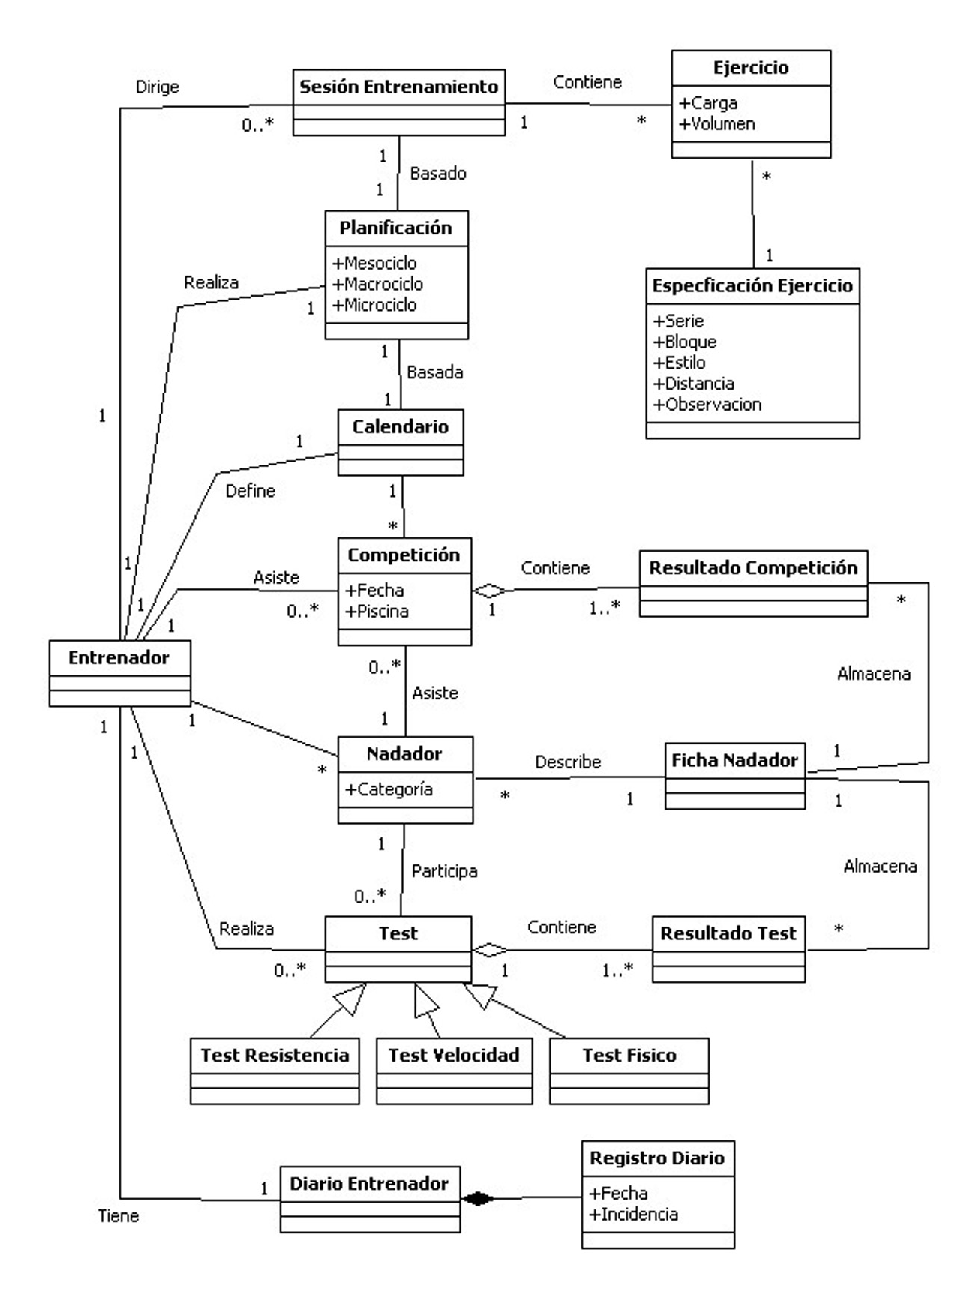
\includegraphics[width=400px]{./eps/captreq_modelo_dominio.eps}
	  \caption{Diagrama del modelo del dominio}
	  \label{fig:modelo_dominio}
	\end{figure}
	
	El recurso activo más importante en un equipo de natación son los nadadores. Los entrenadores dirigen grupos de nadadores agrupados por categorías, ayudando ello a que se puedan aplicar metodologías de entrenamientos a grupos homogéneos. Es cierto que, a pesar de que este sea el caso ideal, no siempre es posible. Hay veces en los que hay que agrupar a nadadores de diferentes edades para formar grupos. Los ejemplos más comunes que ocasionan esta situación son: la falta de espacio en las instalaciones donde se realizan las sesiones de entrenamientos o la falta de nadadores, debido a que es un equipo pequeño. Estas razones son las causantes de que en el modelo del dominio se exprese que un entrenador puede dirigir a cualquier nadador, independientemente de la categoría a la que pertenezca.
	
	Para controlar a cada nadador, el entrenador genera fichas que describen a cada uno de los nadadores. En ella se almacenan los datos personales, los datos de contacto y resultados obtenidos en test o competiciones. Sobre esto se hablará posteriormente.
	
	Al principio de una temporada y orientado a un grupo de nadadores, el cuerpo técnico realiza una planificación deportiva. El entrenador define un calendario con las competiciones a las cuales se asistirá, lo que conlleva que se marquen las pautas para definir los periodos de una planificación. Entiéndase por periodos la definición de macrociclos, mesociclos y microciclos.
	
	\begin{itemize}
		\item{{\bf Microciclo} es un conjunto de sesiones que tienen un objetivo concreto. Como su nombre indica, son ciclos breves de entrenamiento. Comúnmente, los microciclos hacen referencia a cada sesión de entrenamiento que realice un entrenador.}
		\item{{\bf Mesociclos} son bloques de microciclos {\bf ordenados} para conseguir un objetivo determinado: representan etapas relativamente acabas del proceso de entrenamiento que permiten asegurar el desarrollo de una capacidad.}
		\item{{\bf Macrociclo} es un bloque de mesociclos. La idea equivale al concepto de periodo de entrenamiento, los que normalmente suelen ir separados por reposos. } 
	\end{itemize}
	
	Uno de los fines de la planificación es obtener unos niveles de carga y volumen de cada microciclo, o lo que es lo mismo, especificar qué cantidad de metros y a qué intensidad se tienen que realizar cada una de las sesiones de entrenamientos. Es por ello, por lo que una sesión de entrenamiento contiene varios ejercicios de distinta tipología. Cada ejercicio refleja la capacidad que se trabaja, siendo los ejercicios aeróbicos \footnote{Aeróbicos incluyen cualquier tipo de ejercicio que se practique a niveles moderados de intensidad durante periodos de tiempo largos.}, anaeróbicos \footnote{Anaeróbicos comprenden actividades breves basadas en la fuerza.} y de técnica \footnote{La técnica hace referencia a la mejora de cada uno de los estilos de natación.} los más usuales.
	
	La especificación de cada ejercicio normalmente está compuesta por bloques, series, distancia, estilo que se nada y detalles más precisos que en el modelo se engloban como {\it observación}. Un ejemplo es {\it 2x(4x100 Mariposa) técnica variada}, el cuál expresa que se realicen 2 bloques de 4 series de 100 metros mariposa, haciendo ejercicios variados de distinta técnica. Esto sumaría un volumen total de 800 metros, generando una carga que se calcula a partir de un parámetro denominado {\it ``índice de Mujika''}.
	
	Por otro lado, otro de los fines de la planificación es preparar a los nadadores para las competiciones que se realicen y a las que se hayan decidido asistir. Por ello, se puede decir tanto entrenadores como nadadores asisten a alguna competición celebrada en una fecha y piscina determinada. Es importante reflejar la piscina, puesto que éstas pueden ser de 25 o 50 metros de longitud. Es lógico preguntarse, ¿en qué influye en el nadador la longitud de la piscina? Un nadador recorriendo una misma distancia en piscinas de 25 y de 50 metros, realiza un tiempo total distinto. 
	
	Dejando de lado una explicación técnica que explique el motivo, se puede afirmar que en una competición, un nadador puede realizar diferentes pruebas, lo que ocasionaría en una batería de resultados a almacenar en su ficha. El conjunto de todos los resultados de cada competición por cada nadador, forman la relación {\it Competición---Resultado competición}.
	
	Debido a que en el control está el éxito, para comprobar las capacidades de cada nadador, un entrenador realiza diferentes pruebas o {\it test}. Éstos pueden ser de diferente tipo, siendo los principales los que miden la resistencia, velocidad y otras capacidad físicas (tales como envergadura, talla o peso). Estas pruebas se realizan a lo largo de la temporada, obteniendo resultados que se almacenan también en la ficha del nadador.
	
	Por último, cada entrenador tiene un diario en el que registra las incidencias o sucesos que ocurren a lo largo de una temporada. Aporta información en una etapa de {\it feedback} \footnote{La realimentación, también denominada retroalimentación o feedback, significa ‘ida y vuelta’ y es, desde el punto de vista social y psicológico, el proceso de compartir observaciones, preocupaciones y sugerencias, con la intención de recabar información, a nivel individual o colectivo, para intentar mejorar el funcionamiento de una organización o de cualquier grupo formado por seres humanos.}, donde lo que importa es observar los sucesos del pasado para mejorar el proceso de entrenamiento (posibles cambios en el proceso de realización de planificación, ver como funciona un determinado ejercicio sobre una categoría o anotar competiciones a las que no ir en temporadas próximas son ejemplos de datos a añadir en el diario).    
	% -----------------------------------------------------------------------------
	%  NOTA: Añadir al modelo de dominio los tipos de ejercicios e índice e Mujika
	%	Corregir tilde de Especificación de Ejercicio -> observación
	% -----------------------------------------------------------------------------

	
% subsection construcción_del_modelo_del_dominio (end)

% section modelo_del_dominio (end)

% chapter captura_de_requisitos (end) % Captura de requisitos
	
	% ----------------- Glosario --------------------------- 
	% Para mostrar todas las entradas aunque no estén referenciadas en el documento
	\newgloss{default}{.gls}{Glosario de términos}{glsplain}
	\gloss[nocite]{*} 		
	\printgloss{glsbase,glosario}

	% ----------- Referencias bibliograficas ------------------ 
	\nocite{*}	% Se usa para indicar en la bibliografia las referencias no citadas.
	\bibliography{bibliografia}
	\bibliographystyle{plain}
	
\end{document}
